\section{Question 1: Weighted Household Utility}\label{sec:q1}

\subsection*{Model}

In the baseline model the household utility is an equal-weighted sum of the two members' utilities:
%
\begin{equation}\label{eq:baseline_util}
    U(c_t, h_{1,t}, h_{2,t}) = 2\frac{(c_t/2)^{1+\eta}}{1+\eta} - \rho_1 \frac{h_{1,t}^{1+\gamma}}{1+\gamma} - \rho_2 \frac{h_{2,t}^{1+\gamma}}{1+\gamma}
\end{equation}
%
We assign the weight $\mu \in [0,1]$ to member 1 and $(1-\mu)$ to member 2. Writing the individual utilities as
%
\begin{equation}
    u_j(c_t, h_{j,t}) = \frac{(c_t/2)^{1+\eta}}{1+\eta} - \rho_j \frac{h_{j,t}^{1+\gamma}}{1+\gamma}, \quad j \in \{1,2\},
\end{equation}
%
the weighted household utility is the convex combination
%
\begin{equation}\label{eq:weighted_util}
    U(c_t, h_{1,t}, h_{2,t}) = \mu \, u_1(c_t, h_{1,t}) + (1-\mu) \, u_2(c_t, h_{2,t}).
\end{equation}
%
Since $\mu + (1-\mu) = 1$, this expands to
%
\begin{equation}
    U = \frac{(c_t/2)^{1+\eta}}{1+\eta} - \mu \, \rho_1 \frac{h_{1,t}^{1+\gamma}}{1+\gamma} - (1-\mu) \, \rho_2 \frac{h_{2,t}^{1+\gamma}}{1+\gamma},
\end{equation}
%
so member~1 carries the labor-disutility weight $\mu$ and member~2 the weight $(1-\mu)$.

\subsection*{Implementation}

We add the parameter \texttt{par.mu = 0.5} to the model class. In \texttt{util()} the labor disutility of member~1 is weighted by \texttt{par.mu} and that of member~2 by \texttt{1-par.mu}, with consumption entering as \texttt{(cons/2)**(1+eta)/(1+eta)}.

At $\mu = 0.5$ the weighted utility is a positive rescaling of the baseline (see Question~2), and because utility is ordinal the optimal labor supply is unaffected. Solving and simulating both specifications confirms this: the average hours coincide down to the optimizer's numerical tolerance,
%
\begin{align*}
    \max|\Delta h_1| &= 9.75\times 10^{-5} \\
    \max|\Delta h_2| &= 1.03\times 10^{-4}.
\end{align*}

\begin{figure}[H]
    \centering
    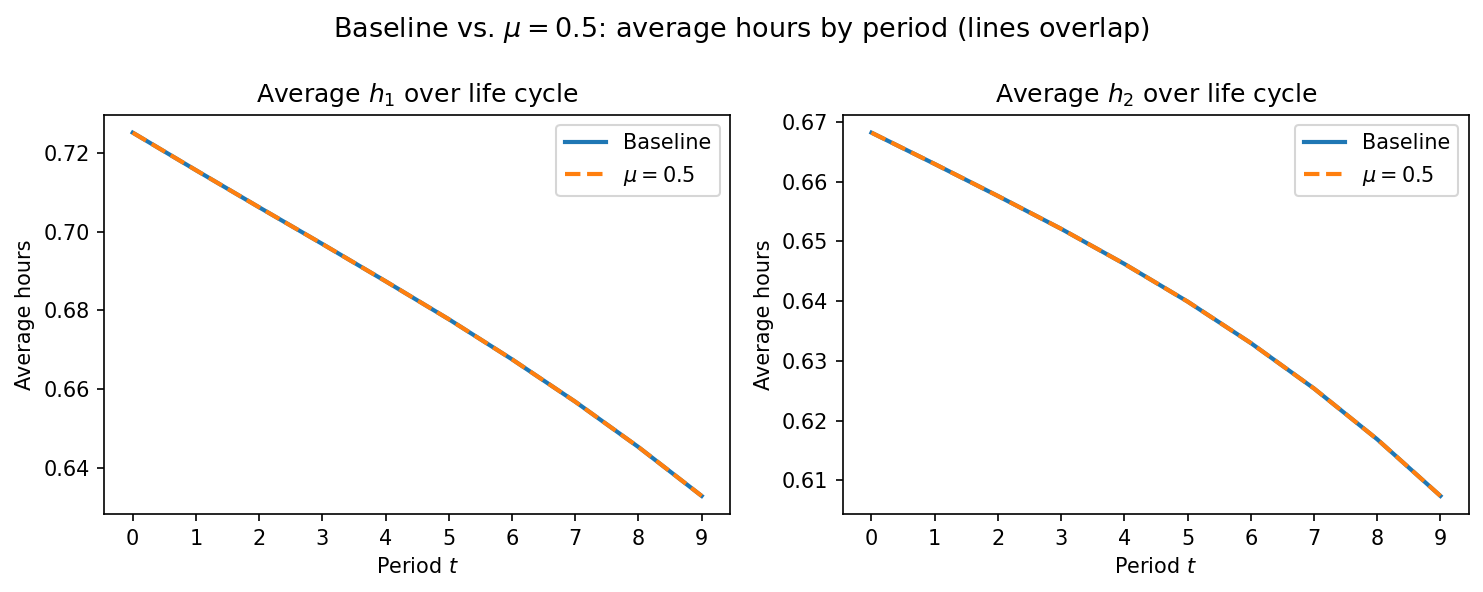
\includegraphics[width=1\linewidth]{Billeder/Baseline_vs_mu05_hours.png}
    \caption{Average hours per period under the baseline and $\mu = 0.5$; the lines overlap.}
    \label{fig:q1_hours}
\end{figure}
